
\chapter{Návrh systému} 
\label{kap:návrh systému}
\pagestyle{fancy}
\fancyhf{}
\fancyfoot[CE,CO]{\thepage}
\renewcommand{\footrulewidth}{1pt}
\lhead{Návrh systému}


\section{Výber kamier}

\subsection{Intel Realsense SR300}

Táto kamera pracuje na princípe SLS a predstavuje vylepšenú verziu staršej Intel RealSense F200. Ide o cenovo dostupnú hĺbkovú kameru, ktorá sníma hĺbku v rozsahu od $0.2-1.5 m$. Poskytuje dynamické snímanie scény pri nízkej spotrebe (napájanie cez USB). V kombinácií s farebným obrazom ($1920\times1080p$, $30Hz$) a hĺbkovou mapou ($640x480p$) ide o jednu z najlepších dostupných SLS kamier na trhu. 

\begin{figure}[H]
	\centering
	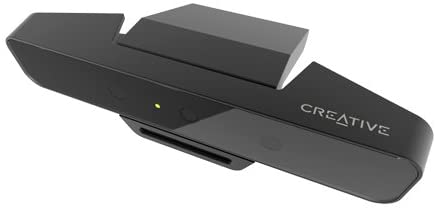
\includegraphics[width=0.7\textwidth]{figures/sr300.jpg}
	\caption{SLS kamera Intel RealSense SR300.}
	\label{fig::sr300}
\end{figure}

Táto kamera obsahuje RGB senzor, IR laserový projektor, IR prijímač a mikrofón. Detailnejšie opísanie princípu SLS je v podkapitole \ref{sec:sls}.

\subsection{Microsoft Kinect v2}

Ide o druhú generáciu hĺbkových kamier od spoločnosti Microsoft. Oproti prvej generácií využíva technológiu ToF (detailnejšie v \ref{sec:tof}), pričom ide o jednu z najznámejších senzorov tohto typu na svete. Rozsah snímanej scény je $0.5-4.5 m$. Farebný obraz je dodávaný v rozlíšení $1920\times1080p$ a $30Hz$, hĺbková mapa ma rozlíšenie $512\times424$.

\begin{figure}[H]
	\centering
	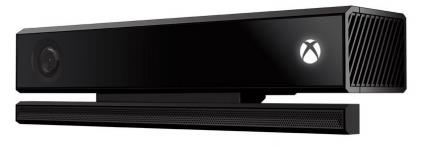
\includegraphics[width=0.7\textwidth]{figures/kinect.png}
	\caption{ToF kamera Microsoft Kinect v2.}
	\label{fig::kinect}
\end{figure}

Presnosť hĺbkovej mapy je oproti prvej verzii Kinectu vyššia, taktiež je znížený negatívny vplyv spôsobovaný slnečným svetlom.


\subsection{Porovnanie presnosti kamier}

Cieľom testovania bolo porovnať presnosť 3D rekonštrukcie statického objektu pre kamery Intel RealSense SR300 a Microsoft Kinect v2. Pomocou programov, určených k práci s jednotlivými kamerami, bola vytvorená séria snímok hĺbkových máp a ich rekonštruovaných 3D modelov. Pred snímaním bola vykonaná geometrická kalibrácia kamier, ktorej technické detaily sú opísané v kapitole \ref{sec:kinect_calib}. Kalibrovanými kamerami sa následne z 3 uhlov (pohľady spredu, z ľavej a pravej strany) získali ich 3D rekonštrukcie, ktoré zachytávali všetky potrebné detaily pre meranie. Identické natočenie pre obe kamery bolo zabezpečené rotačným podstavcom. 

\begin{figure}[H]
	\centering
	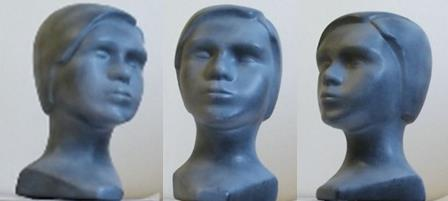
\includegraphics[width=0.7\textwidth]{figures/rgb_compar.png}
	\caption{ToF kamera Microsoft Kinect v2.}
	\label{fig::rgb_compare}
\end{figure}

Povrch objektu bol špeciálne upravený, aby nevytváral odlesky spôsobujúce zhoršovanie rekonštruovaného 3D modelu. 

\section{Snímanie dynamických objektov}

Pri snímaní dynamických objektov je potrebné uvažovať so vznikom pohybových artefaktov. Tie vznikajú, ak objekt v dobe skenovania mení svoje priestorové umiestnenie. Z toho dôvodu je potrebné buď stabilizovať objekt počas doby snímania alebo redukovať časovú dĺžku skenovania. Keďže tento systém má byť určený pre medicínske aplikácie, kde skenovaný objekt bude pediatrický pacient, je potrebné overiť možnosti experimentálne.


\subsection{Jedno-kamerové snímanie dynamických objektov}

Experimentálne snímanie pacientov bolo vykonávané na Klinike detí a dorastu Jesseniovej lekárskej fakulty v Martine, Laboratórium spánkovej medicíny. Do testu bolo vybraných 9 pacientov rôzneho pohlavia,vo vekovom rozmedzí od 4 do 12 rokov. 

Ako skenovací nástroj bola použitá kamera Kinect v2. V spolupráci s komerčným softvérom KScan3D boli vytvorené modely pacientov, ktoré sú zobrazené na obr. \ref{fig:dynamic_patient:a} a \ref{fig:dynamic_patient:b}. 

\begin{figure}[H]
	\centering
	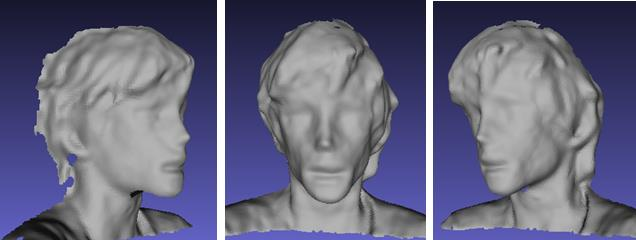
\includegraphics[width=\textwidth]{figures/dynamic_patient_a.png}
	\caption{ToF kamera Microsoft Kinect v2.}
	\label{fig:dynamic_patient:a}
\end{figure}

\begin{figure}[H]
	\centering
	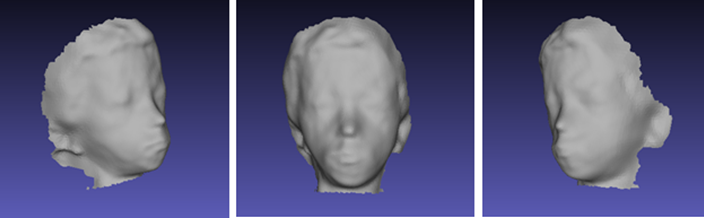
\includegraphics[width=\textwidth]{figures/dynamic_patient_b.png}
	\caption{Úkažka .}
	\label{fig:dynamic_patient:b}
\end{figure}

Ako je vidieť, modely sú nekvalitné a výrazne deformované. Je to spôsobené tým, že objekty nedokázali zostať v statickej polohe počas doby skenovania (tá presahovala 1 minútu pri každom pacientovi). Tendenciou bolo otáčať sa za kamerou, čo viac krát viedlo k nutnosti začas celý proces od znova. 

Takéto modely nie su postačujúce pre diagnostikovanie OSAS. Ich miera nepresnosti je veľmi vysoká a užitočná geometria tváre sa stráca. Z experimentu vyplýva, že jedno-kamerový systém je nepoužiteľný pre skenovanie dynamických objektov ako sú pediatrickí pacienti.  

\subsection{Priestorové rozloženie multi-kamerového systému}

Pri multi-kamerovom systéme sa pre skenovanie používajú viaceré kamery, ktoré su staticky rozložene v priestore. Ich počet závisí od detailov objektu, ktoré majú byť zosnímané.

\begin{figure}[H]
	\centering
	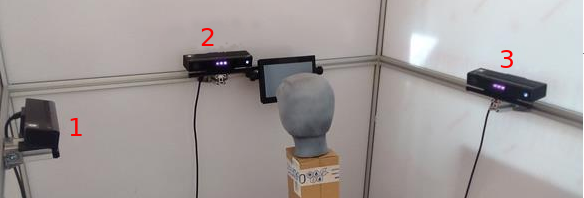
\includegraphics[width=0.6\textwidth]{figures/multicam_placement.png}
	\caption{Úkažka .}
	\label{fig:multicam:placement}
\end{figure}


Medzi hlavné požiadavky na model sú: hlava musí obsahovať laterálne pohľady (umožniť prekrytie s cefalometrickou snímkou) a orientačné bodov mäkkého tkaniva. Dôležité je aj získanie informácie o šírke krk. Na obrázku \ref{fig:multicam:placement} je zobrazené rozloženie kamier v skenovacej kabíne. Ich jednotlivé 3D modely aj s verifikáciou požiadaviek sa nachádzajú na obr. \ref{fig:multicam:models}. 

\begin{figure}[H]
	\centering
	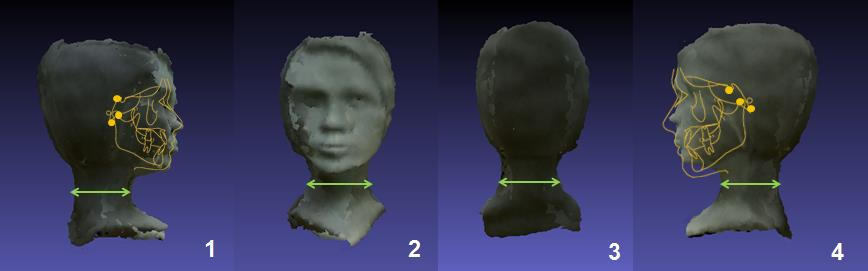
\includegraphics[width=\textwidth]{figures/multicam_placement_scans.png}
	\caption{Úkažka .}
	\label{fig:multicam:models}
\end{figure}

\subsection{Sekvenčné snímanie multi-kamerového systému}

Sekvenčný mód predstavuje postupné snímanie. V jednom momente vždy sníma len jedna kamera ostatné kamery sú vypnuté. Tento režim je pri ToF kamerách často využívaný, pretože tu nevzniká multi-kamerová interferencia. Problémom je však dlhá doba zapínania IR projektora, ktorá pri kamerách Microsoft Kinect v2 dosahuje približne $1s$. Časový odstup medzi dvoma prijatými snímkami je pri $30Hz$ okolo $33ms$.

\subsection{Paralelné snímanie multi-kamerového systému}

V paralelnom režime pracujú všetky kamery v rovnakom čase. Oproti sekvenčnému snímaniu sa inicializácia vykonáva pre každú kameru iba raz. Tým sa radikálne znižuje doba snímania objektu zo všetkých uhlov. Nevýhodou je ale vznik multi-kamerovej interferencie, ktorá dokáže negatívne ovplyvniť výstupné hĺbkové mapy. Časový rozostup medzi jednotlivými snímkami je ovplyvnení samotným spracovaním dát, maximálne však $33ms$ medzi všetkými snímkami. 

\subsection{Porovnanie režimov snímania dynamických objektov}
\label{sec:serial_parallel}
Pre porovnanie týchto režimov bol navrhnutý experiment, pri ktorom sa porovná veľkosť zmeny polohy objektu v závislosti na dĺžke snímania. Pre testovanie bol vyrobený merací prvok, ktorý pozostával z jednosmerného motora, ukazovateľa aktuálnej polohy a statického podstavca slúžiaceho ako uhlomer. Na hriadeli motora bol pripevnený ukazovateľ, ktorý vykonával pohyb po kružnici. Rýchlosť bola nastavená na regulovateľným zdrojom tak, aby otočka trvala $5s$. Obvod statického podstavca bol rozdelený na 36 dielov oddelených od seba po $10^\circ$. Kvôli identifikácii polohy podstavec obsahoval zvýraznený nultý bod a šípku informujúcu o smere otáčania ukazovateľa.  

\begin{figure}[h]
	\centering
	\begin{subfigure}[b]{\textwidth}
		\centering
		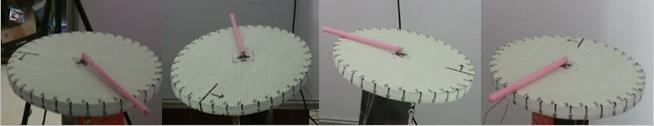
\includegraphics[width=\textwidth]{figures/dynamic_sequence.png}
		\label{fig:dynamic:sequence}
	\end{subfigure}
	\vfill
	\begin{subfigure}[b]{\textwidth}
		\centering
		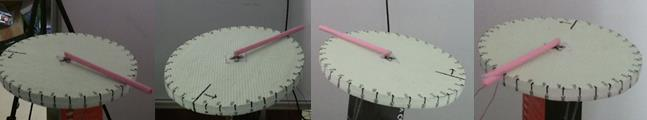
\includegraphics[width=\textwidth]{figures/dynamic_parallel.png}
		\label{fig:dynamic:parallel}
	\end{subfigure}
	\caption{}
	\label{fig:dynamic:results}
\end{figure}

Pri sekvenčnom režime boli snímky z kamier získavané postupne od 1 po 4 kameru. Pri paralelnom režime je ťažké identifikovať poradie. Pre porovnanie bolo potrebné získané hĺbkové mapy previesť na mračno bodov a pomocou ICP metódy ich registrovať do jedného modelu (zhodná pozícia nultého bodu). 

\begin{figure}[h]
	\centering
	\begin{subfigure}[b]{0.42\textwidth}
		\centering
		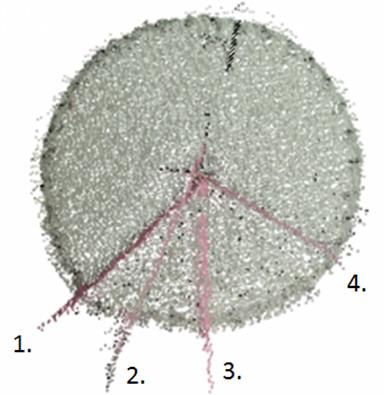
\includegraphics[width=\textwidth]{figures/dynamic_result_seq.png}
		\caption{}
		\label{fig:depthir:a}
	\end{subfigure}
	\hfill
	\begin{subfigure}[b]{0.42\textwidth}
		\centering
		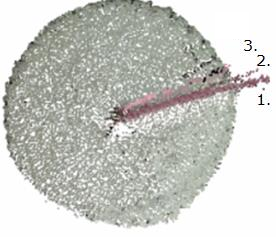
\includegraphics[width=\textwidth]{figures/dynamic_result_par.png}
		\caption{}
		\label{fig:depthir:b}
	\end{subfigure}
	\caption{Obrazy z senzora Microsoft Kinect v2: (\textbf{a}) IR obraz bez interferencie. (\textbf{b}) IR obraz s interferenciou. (\textbf{c}) Hĺbková mapa IR obrazu (a). (\textbf{d}) Hĺbková mapa IR obrazu (b). Miesto interferencie je zvýraznené červenou farbou.}
	\label{fig:depthir}
\end{figure}


\begin{figure}[H]
	\centering
	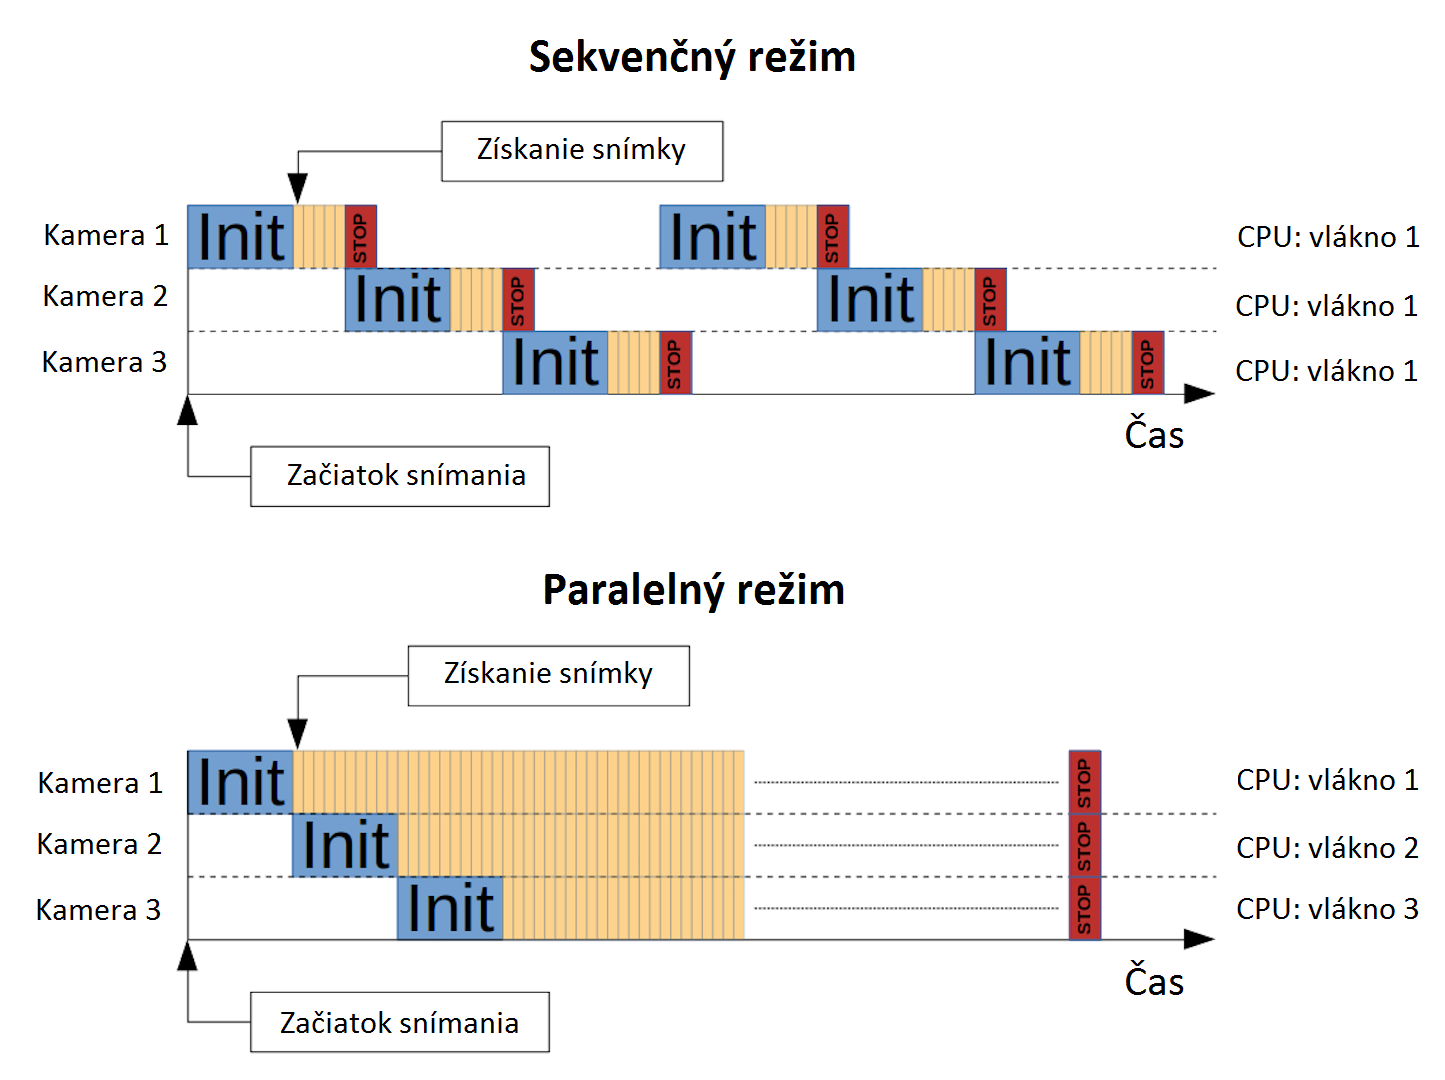
\includegraphics[width=\textwidth]{figures/scanning_mode.png}
	\caption{Úkažka .}
	\label{fig:multicam:models}
\end{figure}

Z výsledných modelov je jasne vidieť, že paralelné spracovanie dát má vyšší zmysel pri snímaní dynamických objektov. Pri sekvenčnom režime je rozdiel polohy ukazovateľa výrazný, čo spôsobovalo problémy aj pri ICP registrácií. Naproti tomu je model vytvorený paralelným režimom konzistentnejší, rozdiel polohy ukazovateľa je podstatne menší. Ten by sa dal znížiť hardvérovým synchronizovaným snímaním. Pri kamerách Kinect v2 však táto možnosť chýba.

\section{Kalibrácia kamier systému}
\label{sec:kinect_calib}
Pre kalibráciu bol použitý \textit{Matlab Calibration ToolBox}. 

\subsection{Geometricka kalibrácia}
Cieľom geometrickej kalibrácie je získanie vnútorných parametrov  kamery spolu s korekčnými parametrami pre odstránenie tangenciálneho a radiálneho skreslenia. Tieto parametre bolo potrebne získať pre RGB aj IR senzory všetkých používaných hĺbkových kamier Kinect v2. 

Pre kalibráciu RGB a IR senzora sa vytvorila séria snímok, ktoré  obsahovali kalibračný vzor snímaný z rôznych uhlov. Ten bol reprezentovaný šachovnicovým motívom o rozmeroch $10\times8$, pričom dĺžka hrany mala veľkosť $36mm$.


%\begin{figure}[h]
%	\centering
%	\begin{subfigure}[b]{0.59\textwidth}
%		\centering
%		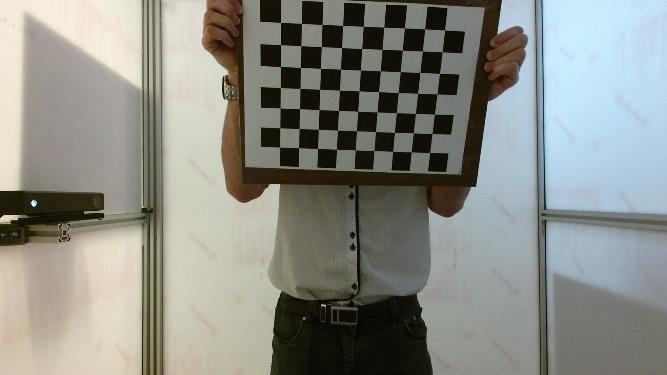
\includegraphics[width=\textwidth]{figures/calibration_rgb.png}
%		\caption{}
%		\label{fig:calib:rgb}
%	\end{subfigure}
%	\hfill
%	\begin{subfigure}[b]{0.4\textwidth}
%		\centering
%		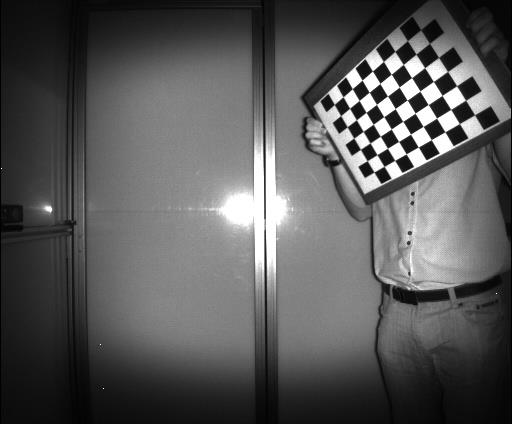
\includegraphics[width=\textwidth]{figures/calibration_ir.png}
%		\caption{}
%		\label{fig:calib:ir}
%	\end{subfigure}
%	\caption{Obrazy z senzora Microsoft Kinect v2: (\textbf{a}) IR obraz bez interferencie. (\textbf{b}) IR obraz s interferenciou. (\textbf{c}) Hĺbková mapa IR obrazu (a). (\textbf{d}) Hĺbková mapa IR obrazu (b). Miesto interferencie je zvýraznené červenou farbou.}
%	\label{fig:calib:single}
%\end{figure}

Pre overenie správnosti kalibrácie IR snímača sa porovnával kalibrovaný kamerový systém s nekalibrovaným voči referenčnému modelu. Pri rovnakých podmienkach prostredia bol zosnímaný model hlavy s továrenskými nastaveniami, potom boli použité kalibračné koeficienty získané v predchádzajúcom kroku. Referenčný model bol vytvorený ručným laserovým skenerom. Ukážky sa nachádzajú na obr. \ref{fig:calib:models}. 

\begin{figure}[H]
	\centering
	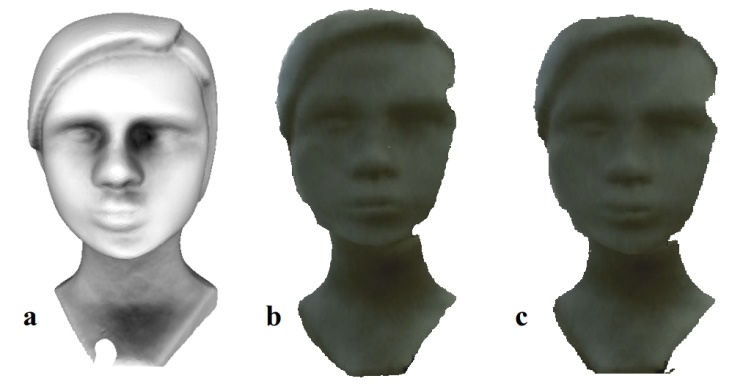
\includegraphics[width=0.6\textwidth]{figures/calibration_models.jpg}
	\caption{}
	\label{fig:calib:models}
\end{figure}

Porovnanie priestorovej rekonštrukcie hĺbkových máp bolo robené pomocou Hausdorffovej vzdialenosti. V nej je detailnejšie zobrazené, aký vplyv má kalibrácia na generované dáta. Z modelu vzdialenosti (obr. \ref{fig:calib:haus:single}) je vidieť, že nekalibrovaný systém vykazoval vyššiu chybu na okrajoch modelu. To je spôsobené pozitívnym radiálnym skreslením IR senzora, ktorého intenzita je výraznejšia na okrajoch obrazu. Štatistické výsledky pre 10 modelov sa nachádzajú v tabuľke \ref{tab:calib:single}.

\begin{figure}[H]
	\centering
	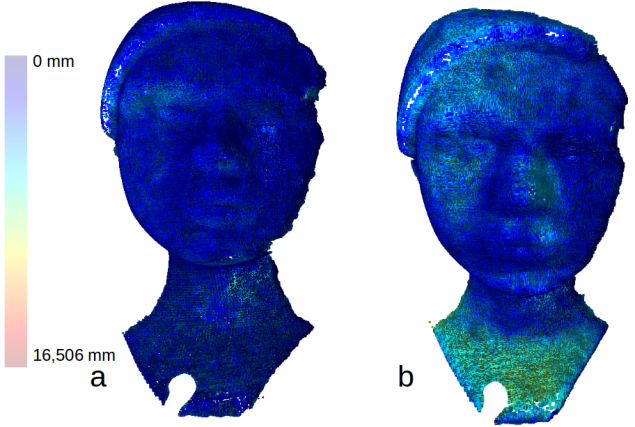
\includegraphics[width=0.52\textwidth]{figures/calibration_hausdorff_single.jpg}
	\caption{}
	\label{fig:calib:haus:single}
\end{figure}



\begin{table}[h]
	\caption{\label{tab:calib:single} Štatistické porovnanie geometrickej kalibrácie kamier }
	\centering
	\begin{tabular}{cccc}
		\toprule
		\textbf{Model} & \textbf{Počet bodov [-]} & \textbf{Mean [mm]} & \textbf{RMS [mm]} \\ 
		\midrule
		\textbf{Nekalibrovaný} & 185187 & 3,0206	& 3,8444 \\
		\textbf{Kalibrovaný} & 296585   & 2,1832   & 2,9506  \\  
		\bottomrule
	\end{tabular}
\end{table}

Týmto krokom sa overil spôsob geometrickej kalibrácie hĺbkových máp. V systéme, kde sa využíva viacero kamier a je kladený dôraz na precíznosť rekonštrukcie, ide o nevyhnutný krok. 


\subsection{Multi-kamerová kalibrácia}

V tomto procese sa odhadujú vzájomné pozície staticky umiestnených kamier vo svetovej súradnicovej sústave. Ich vzájomnú pozíciu určujú rotačné a translačné parametre (kombinácia afinných transformácií z kapitoly \ref{sec:afine}). Tie je možné získať viacerými spôsobmi. Dôležité je si určiť referenčnú kameru, ktorej matica vonkajších parametrov bude mať tvar identickej afinnej transformácie. Pri multi-kamerovej kalibrácií sa využíva podobný postup ako pri geometrickej kalibrácii. Rozdielom je však, že sa kalibračný vzor sníma súčasne z viacerých kamier. Problém nastáva, ak ich rozloženie neumožňuje súčasné snímanie. Takýto prípad je zachytený na obr. \ref{fig:multicam:placement}.

Riešením je separátne kalibrovanie medzi susednými kamerami (napr. 1-2, 1-3 a 2-4 alebo 3-4). V tomto procese sa vytvorí séria RGB-D párov snímok z jednotlivých dvojíc. Snímky obsahujú rovnaký kalibračný vzor so šachovnicovým motívom. Dôležité je, aby bol vzor staticky umiestnený a nevznikol polohový posun vo dvojici RGB-D mapy. 


\begin{figure}[H]
	\centering
	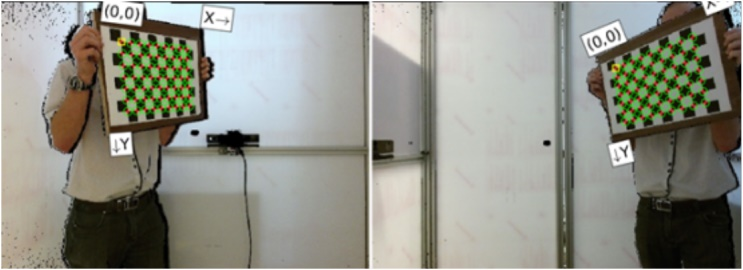
\includegraphics[width=0.7\textwidth]{figures/calibration_multi_rgbd.jpg}
	\caption{}
	\label{fig:calib:multi:rgbd}
\end{figure}

Efektívnejším spôsobom je hľadanie vzájomnej pozície kamier cez kľúčové body. V takomto prípade každá staticky umiestnená kamera zosníma kalibračný objekt, z ktorého vygeneruje mračno bodov. V každom mračne sa identifikujú spoločné body, ktoré slúžia na prvotné zarovnanie. Následne sa ICP metódou minimalizuje suma štvorcov euklidovských vzdialeností bodov. Výhodou statického rozmiestnenia kamier je, že ju je nutné vykonať iba raz. Získaním rotačných a translačných parametrov pre každú kameru získavame zarovnané mračná v spoločnom projektovanom priestore. 

\begin{figure}[H]
	\centering
	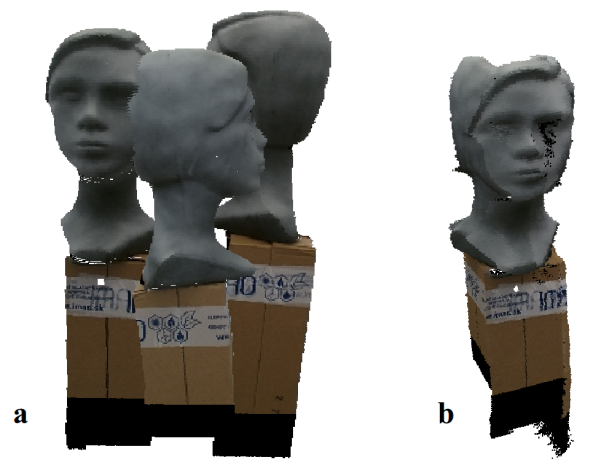
\includegraphics[width=0.52\textwidth]{figures/calibration_multi.jpg}
	\caption{}
	\label{fig:calib:haus:single}
\end{figure}

\begin{figure}[H]
	\centering
	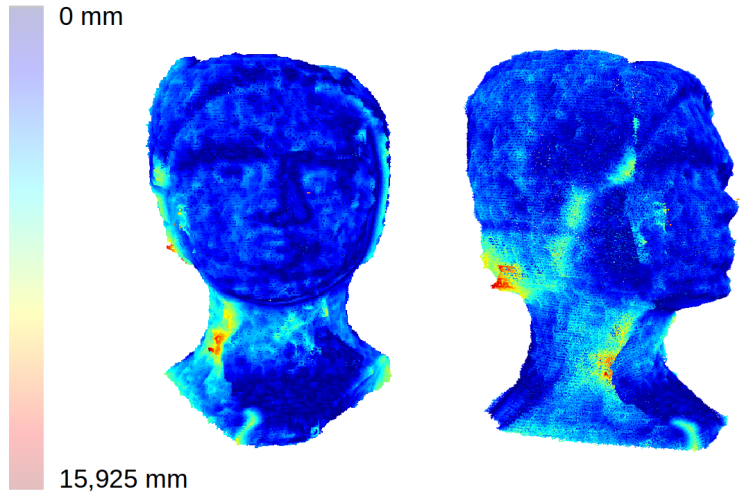
\includegraphics[width=0.52\textwidth]{figures/calibration_hausdorff_multi.jpg}
	\caption{}
	\label{fig:calib:haus:single}
\end{figure}


\section{Návrh algoritmu}

Úlohou algoritmu je vytvoriť konzistentné mračno bodov dynamického objektu z multi-kamerového systému a následne segmentovať parciálne časti mračna podľa preddefinovanej klasifikácie. Dynamický objekt je reprezentovaný hlavou pediatrického pacienta, čiže ide o špecifickú aplikáciu určenú pre medicínske využitie. Cieľom je získať model hlavy pacienta, z ktorého bude možné identifikovať zhluky bodov jednotlivých časti tváre (oči, nos, brada, ústa,...). Takto segmentované body budú v ďalšom výskume použité ako vstupné množiny do neurónových sieti pracujúcich s 3D dátami. \newline

Proces snímania môžeme rozdeliť na 3 fázy. 

\begin{description}[leftmargin=*,labelsep=5.8mm, font=$\bullet$~\normalfont\scshape\color{black!20!black}]
	\item[Príprava dát v reálnom čase]
	\item[Identifikácia polohy hlavy] 
	\item[Segmentácia bodov podľa klasifikácie]
\end{description}


V prvej sa rieši zber dát zo všetkých pripojených kamier. Vykonáva sa 2D a 3D filtrácia, kalibrácia a zarovnávanie mračien bodov. Požiadavka na tento proces je, aby bol vykonávaný v reálnom čase. Ak frekvencia snímania je $30Hz$, časový rozstup medzi snímkami je $33ms$. Preto sú procesy spúšťané paralelne na CPU a GPU. \newline

V druhej fáze sa zabezpečuje uloženie série dát z jednotlivých kamier v statickej pozícii objektu. Táto fáza začína požiadavkou pre zachytenie scény od užívateľa systému. Algoritmus hľadá sériu snímok, kedy dynamický objekt vykonával minimálny pohyb. Počet snímkov v sérii je zadefinovaný v kapitole \ref{kap:interference}, kde je potrebné naplniť obrazový zásobník kvôli potlačeniu multi-kamerového rušenia. Týmto krokom sa minimalizuje vznik pohybových artefaktov vo výslednom mračne bodov. \newline

V poslednej fáze sa vykonáva segmentácia výstupných RGB-D obrazov, v ktorých sa hľadajú regióny prislúchajúce jednotlivých častiam ľudskej tváre. Takouto segmentáciou v 2D  obraze sa následne dokážu identifikovať body v 3D priestore. Táto fáza už nie je vykonávaná v reálnom čase ale ide o post-processing, ktorého spracovanie trvá rádovo niekoľko minút. Výstupom segmentácie sú binárne masky, ktoré klasifikujú jednotlivé regióny v hĺbkových mapách. Pri priestorovej rekonštrukcii sa následne korektným bodom nastaví identifikátor, do ktorej oblasti spadá. Takto je možné rozdeliť jedno zarovnané mračno vytvorené z viacerých hĺbkových máp.

%https://www.researchgate.net/publication/306284947_Efficient_Multi-Frequency_Phase_Unwrapping_using_Kernel_Density_Estimation


\subsection{Príprava vstupných dát}
\label{sec:data_prep}
Proces prípravy vstupných dát môžeme rozdeliť na 4 sekvencie.
V prvom kroku je potrebné inicializovať kamery a nastaviť im správne konfiguračné parametre. Ku komunikácií Kinect v2 s ovládacím programom bol použitý ovládač Kinect v2 s implementovaným CudaKDE algoritmom. Každá kamera má svoje jedinečné sériové číslo, pomocou ktorého je možné správne identifikovať a spárovať výstupy geometrickej a multi-kamerovej kalibrácie. Po úspešnej inicializácii sa všetky kamery zaregistrujú do manažéra procesov. V následnej sekvencii manažér spúšťa paralelné spracovanie dát na CPU, ktoré je oddelené od hlavnej slučky programu. Každá kamera tak nezávisle na sebe prijíma dáta a vykonáva ďalšie spracovanie. Prvým krokom je odstránenie skreslenia šošovky na RGB a IR obraze. Po kalibrácií sa vytvára hĺbková mapa a registráciou RGB obrazu sa získava RGB-D mapa. \newline

Každé vlákno pripravuje vstupné dáta a uchováva si ich po dobu svojej iterácie:

\begin{description}[leftmargin=*, font=$\bullet$~\normalfont\scshape\color{black}]
	\item[RGB:] 	8-bitový 3-kanálový obraz s rozlíšením $1920 \times 1080$
	\item[IR:]	32-bitový šedo-tonový obraz s rozlíšením $512 \times 424$
	\item[Depth:] 32-bitový šedo-tónový obraz s rozlíšením $512 \times 424$
	\item[RGB-D:] 8-bitový 3-kanálový obraz s rozlíšením $512 \times 424$
\end{description}

Po úspešnej kolekcii vstupných dát manažér procesov zabezpečí bezpečný presun do dátového zásobníka. Úlohou zásobníka je spravovať a aktualizovať potrebné dáta a pravidelne čistiť tie staré. Jeho veľkosť je rekonfigurovateľná, minimálnu hodnotu určujú potreby IMBM filtra. Dátový zásobník sa skladá z obrazových zásobníkov a zásobníkov mračien bodov. 

\begin{figure}[H]
	\centering
	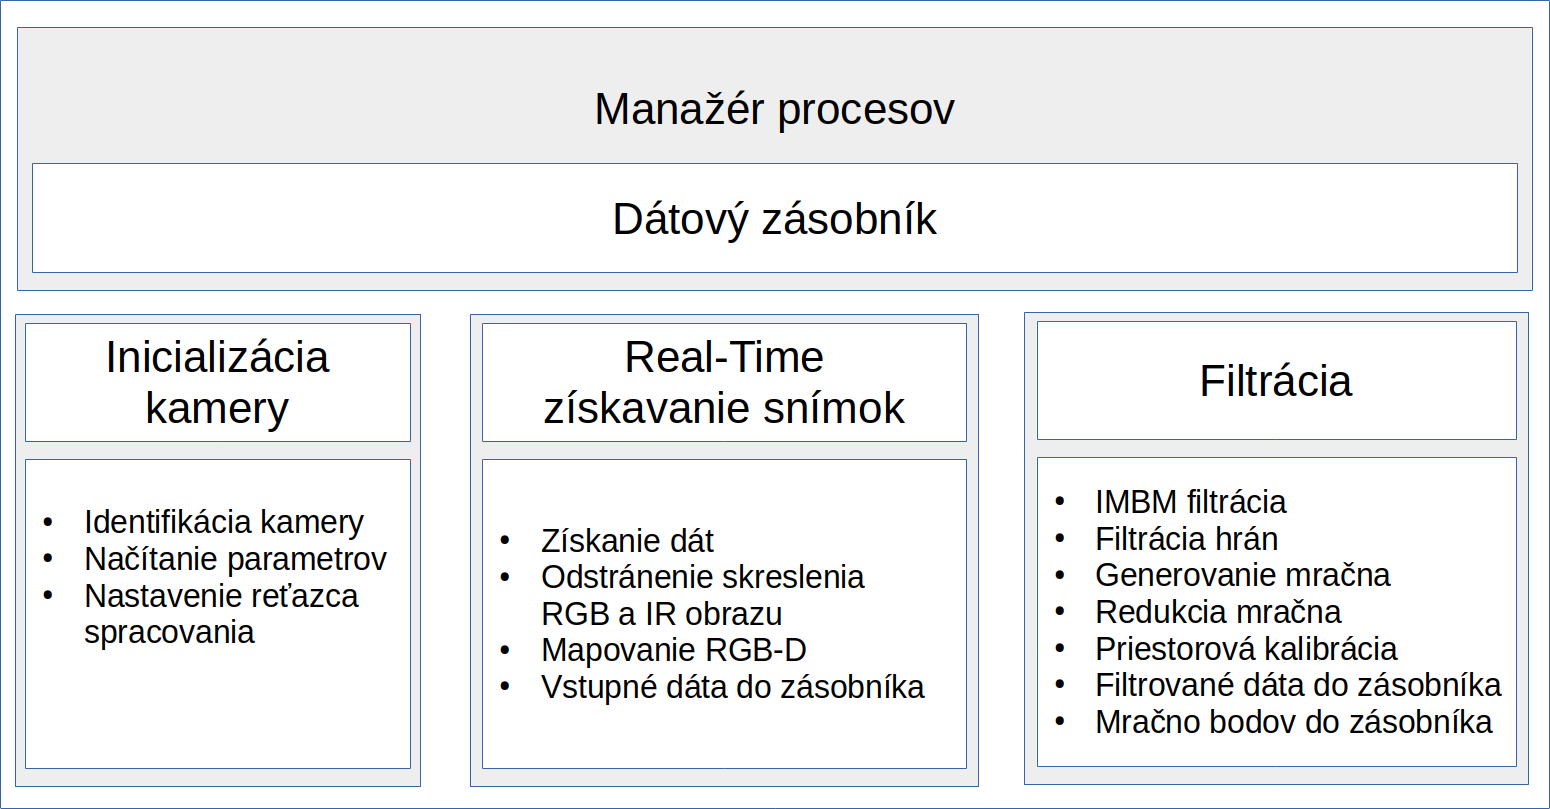
\includegraphics[width=\textwidth]{figures/algorithm_capture.png}
	\caption{}
	\label{fig:algorithm:process:a}
\end{figure}

Po prijatí nových dát z jednotlivých kamier do dátového zásobníka manažér procesov iniciuje filtráciu série hĺbkových snímkov. Filtrácie taktiež bežia v samostatných vláknach CPU. Hlavnou filtračnou metódou je IMBM filter, ktorý zo vstupnej série hĺbkových máp vytvára jednu mediánovú hĺbkovú mapu. V nej je minimalizovaná chyba spôsobená šumom kamery, taktiež sa potláča chyba multi-kamerovej interferencie. Následne sa eróziou odstránia nekvalitné pixely na hranách snímaného objektu. Upravenú hĺbkovú mapu používame na generovanie mračna bodov, pričom priemerná RGB-D mapa, vypočítaná zo série vstupných RGB-D obrazov, sa používa na doplnenie textúry generovaného mračna. Body majú štruktúru XYZRGB. Kvôli rýchlejšiemu spracovaniu sa organizovaná štruktúra bodov (217088 bodov z hĺbkovej mapy) prevádza na 1D pole, čím je možné odstrániť prebytočné body reprezentované 0 hodnotou pixelu v hĺbkovej mape. Takto sa počet bodov môže redukovať až o $90\%$, čím sa výrazne zníži aj výpočtová náročnosť. 

\begin{description}[leftmargin=*, font=$\bullet$~\normalfont\scshape\color{black}]
	\item[Depth median:] 	32-bitový šedo-tónový obraz s rozlíšením $512 \times 424$
	\item[RGB-D median:]	8-bitový 3-kanálový obraz s rozlíšením $512 \times 424$
	\item[Median Point Cloud:] Mračno bodov so štruktúrou XYZRGB 
\end{description}

\begin{figure}[H]
	\centering
	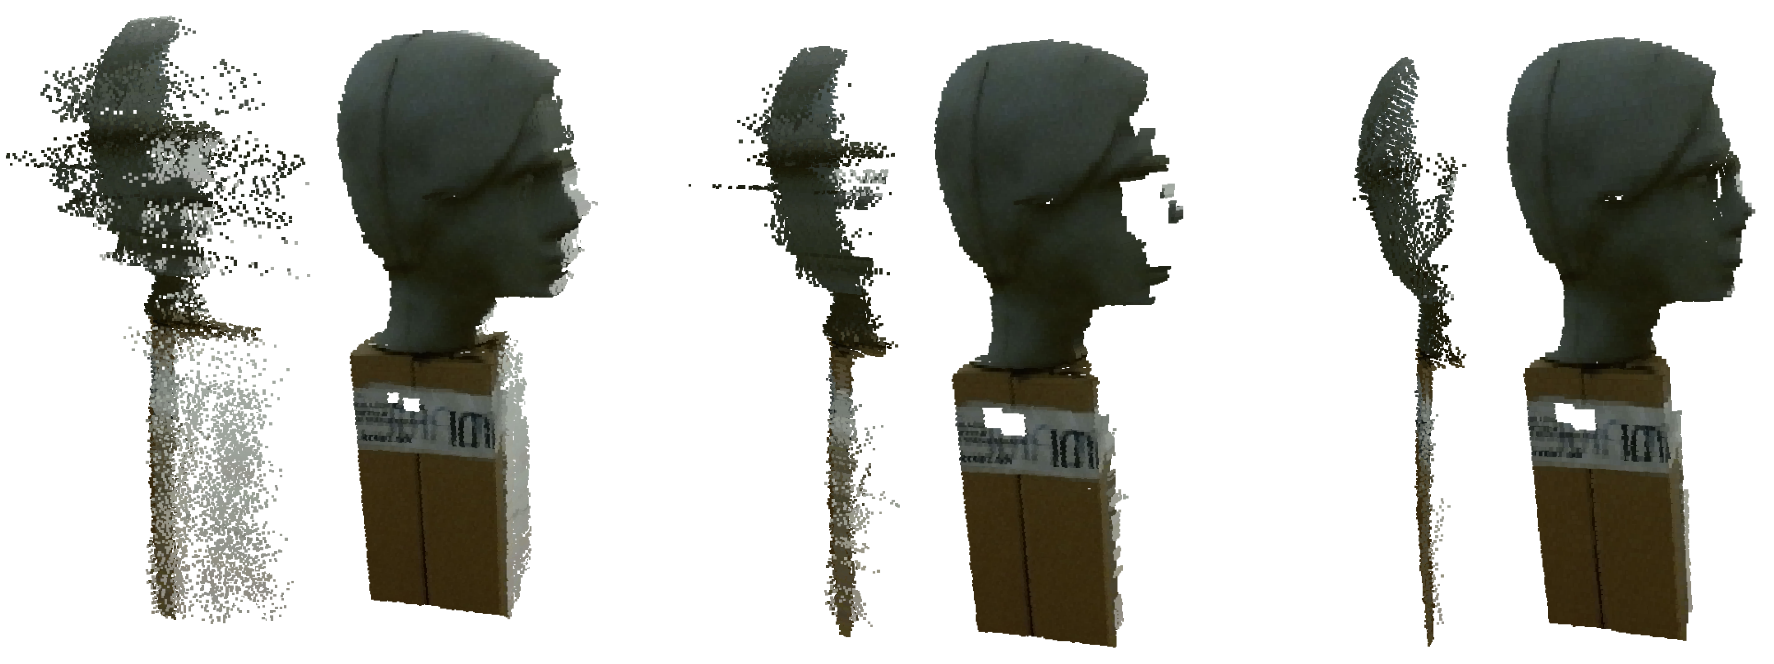
\includegraphics[width=\textwidth]{figures/prepared_models.png}
	\caption{Porovnanie vplyvu filtrácie na vstupné dáta}
	\label{fig:algorithm:result:a}
	\label{fig:algorithm:result:b}
	\label{fig:algorithm:result:c}
\end{figure}

Na obrázkoch je vidieť vplyv filtrácie na vstupné dáta, ktoré sú zašumené a navyše aj interferované. Na obr. je vidieť značnú deformáciu bodov práve v oblasti komplexnejšieho povrchu. Filtráciou sme identifikovali väčšinu interferujúcich dát, ktoré sú v modeli na obr. odstránené. Opravou a interpoláciou poškodených dát sa následne získavalo mediánové mračno bodov, na ktorom sú potlačené deformácie a minimalizované šumy. 

\subsection{Identifikácia polohy hlavy}

Z dôvodov, ktoré sú opísané v sekcii \ref{sec:data_prep} je potrebné ukladať sériu snímok do dátového zásobníka. Z dát v zásobníku sa následne generuje mračno bodov, ktoré má čo najvernejšie reprezentovať snímaný objekt. Problém však nastáva, ak je objekt počas doby snímania dynamický. Pohybom môže vzniknúť problém s následným zarovnaním dát do spoločného modelu. Taktiež je veľmi pravdepodobné, že výsledný model nebude geometricky odpovedať skutočným rozmerom objektu. Vplyv pohybových artefaktov je znázornený na \ref{sec:serial_parallel}. Požiadavkou je nájsť sekvenciu dát, kedy bol pohyb snímaného objektu minimálny. \newline 

Keďže kamery sú staticky umiestnené a zamerané na spoločný centrálny bod, pohyb objektu v hociktorom smere sa prejaví vo všetkých mapách. Tento fakt je rozhodujúci pri návrhu identifikačného systému. Z toho logicky vyplýva, že stačí analyzovať pohyb objektu len z dát jednej kamery. Identifikovanie kľúčových bodov, ktoré budú zhodné pre každú snímku v obrazovom zásobníku, pomôže vypočítať pohyb a rozptyl polohy. \newline

Ak je pixel $P$ reprezentovaný konkrétnym stĺpcom $r_{i}$ a riadkom $c_{i}$, tak bod záujmu $P_{i}$ prestavuje jedinečnú pozíciu v obraze. Index $i$ predstavuje konkrétny kľúčový bod detektora a $N$ snímku v zásobníku. Bodu $P_{i}$ prislúcha informácia o farbe $R_{i};G_{i};B_{i}$ (získanej z RGB-D obrazu) a o hĺbke $d_{i}$ (získanej z hĺbkovej mapy).

\begin{equation}
\label{key}
\begin{aligned}
P_{i}=P\left(r_{i};c_{i}\right)
\end{aligned}
\end{equation}
\begin{equation}
\label{key}
\begin{aligned}
P_{i;N}=P\left(r_{i;N};c_{i;N}\right)
\end{aligned}
\end{equation}
\begin{equation}
\label{key}
\begin{aligned}
P_{i}=R_{i};G_{i};B_{i};d_{i}
\end{aligned}
\end{equation}

Rozptyl polohy kľúčového bodu $P_d$ sa vypočíta ako absolútna hodnota rozdielu maximálnej a minimálnej pozície pixelu v danom smere. 

\begin{equation}
\label{key}
\begin{aligned}
P_d\left(x\right)=\left|  max\lbrace c_{i;N} \rbrace -min\lbrace c_{i;N} \rbrace \right| 
\end{aligned}
\end{equation}
\begin{equation}
\label{key}
\begin{aligned}
P_d\left(y\right)=\left|  max\lbrace r_{i;N} \rbrace -min\lbrace r_{i;N} \rbrace \right| 
\end{aligned}
\end{equation}
\begin{equation}
\label{key}
\begin{aligned}
P_d\left(z\right)=\left|  max\lbrace d_{i;N} \rbrace -min\lbrace d_{i;N} \rbrace \right| 
\end{aligned}
\end{equation}

Úlohou algoritmu je identifikovať, kedy rozptyl bodov $P_d$ v každom smere neprekročí stanovenú hranicu. Identifikácia sa začína interakciou užívateľa systému (doktor) s grafickým prostredím programu. Snímaný objekt musí byť v pokojovom stave a nastavenej pozícii. Pohybová aktivita je znížená vplyvom podporného vizualizačného systému (tablet premietajúcu zaujímavý obsah), ktorého úlohou je udržať pohľad objektu koncentrovaný na jedno miesto. Príklad RGB-D obrazov dynamického objektu, ktoré môžu byť použité na detekciu kľúčových bodov, je na obr. \ref{fig:dlib:views}. 

\begin{figure}[H]
	\centering
	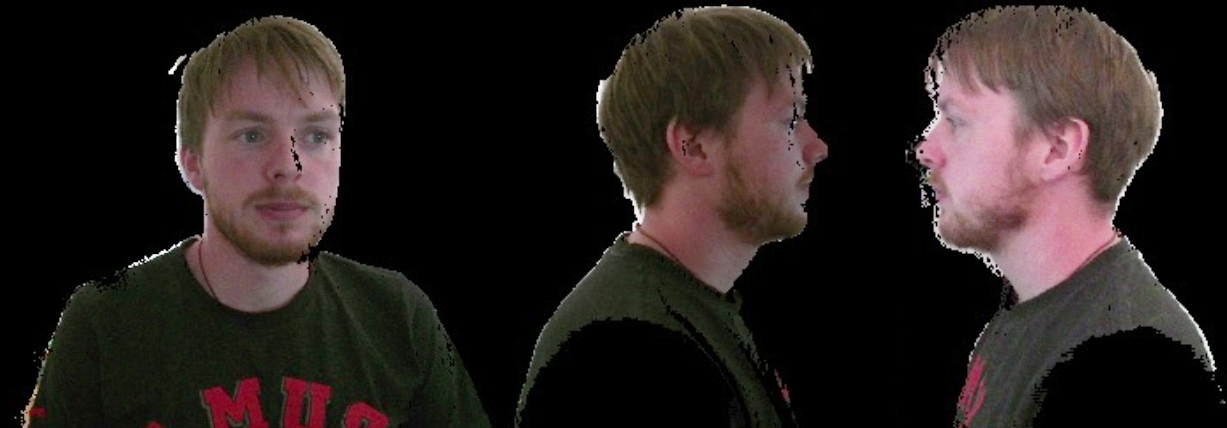
\includegraphics[width=\textwidth]{figures/rgbd_views.png}
	\caption{Aplikácia "DLib Face Landmark Detector":  \textbf{ a)} Označenie 68 základných kľúčových bodov,  \textbf{ b)} Aplikácia na RGB-D obraze získanej z kamery Kinect v2}
	\label{fig:dlib:views}
\end{figure}

Ideálny je frontálny pohľad, pretože tvár obsahuje veľa statických a jedinečných prvkov. V súčasnosti existuje niekoľko desiatok metód, ktoré sú určené na detekciu tváre a jej orientačných bodov. Ich úlohou je čo najpresnejšie identifikovať spomínané body. V tejto práci sa používa detektor DLib, ktorý pracuje na princípe súboru regresívnych stromov.
Základný detektor identifikuje 68 bodov tváre, pričom vie ohraničiť tvár, oči, nos a ústa. Ukážka aplikácie detektora na RGB-D obraze sa nachádza na obrázku \ref{fig:dlib:points}.

\begin{figure}[H]
	\centering
	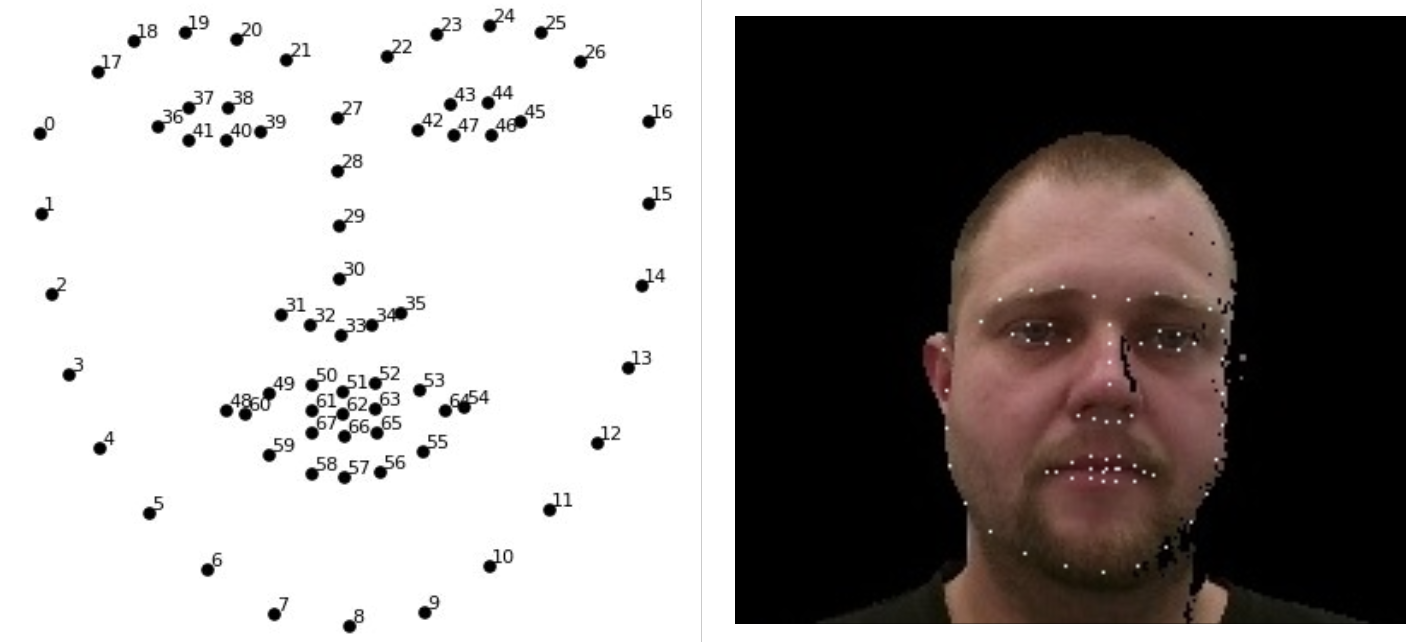
\includegraphics[width=\textwidth]{figures/face_landmarks.png}
	\caption{Aplikácia "DLib Face Landmark Detector":  \textbf{ a)} Označenie 68 základných kľúčových bodov,  \textbf{ b)} Aplikácia na RGB-D obraze získanej z kamery Kinect v2}
	\label{fig:dlib:points}
\end{figure}
 
Problém nastáva pri chýbajúcich dátach v RGB-D obraze, ktoré vznikajú pri mapovaní RGB obrazu na poškodenú hĺbkovú mapu. Kvôli spracovaniu v reálnom čase je detekcia vykonávaná paralelne s filtráciou. Preto sa k detekcii používajú ešte nefiltrované dáta. Na nich môže dochádzať k nesprávnej detekcii bodov. Problematické su aj body 0 až 16, pretože v závislosti na fenotype tváre sa ich umiestnenie môže vyskytnúť mimo objektu. 

Redukovanie počtu detekovaných kľúčových bodov na minimálny počet zabezpečí zníženie stavu, kedy bod $P_i$ bude mať hodnotu $d_i=0$. K nasledujúcej detekcii bol použitý detektor identifikujúci 5 kľúčových bodov. 
 
\begin{figure}[H]
	\centering
	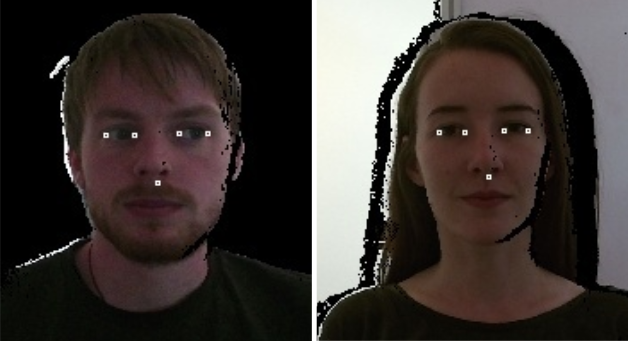
\includegraphics[width=0.75\textwidth]{figures/rgbd_points.png}
	\caption{Porovnanie vplyvu filtrácie na vstupné dáta}
	\label{fig:dlib:rbbd5}
	\label{fig:dlib:rbbd5:b}
\end{figure}

Z RGB-D obrazu (obr. \ref{fig:dlib:rbbd5}) sa následne pozície kľúčových bodov $r_i, c_i$ prenesú do hĺbkovej mapy. Získajú sa hĺbkové informácie $d_i$ a vypočítajú sa hodnoty $P_d$. 

\begin{figure}[H]
	\centering
	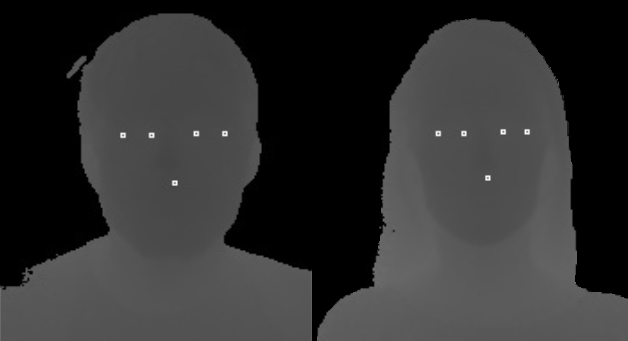
\includegraphics[width=0.75\textwidth]{figures/depth_points.png}
	\caption{Porovnanie vplyvu filtrácie na vstupné dáta}
	\label{fig:algorithm:result:a}
	\label{fig:algorithm:result:b}
	\label{fig:algorithm:result:c}
\end{figure}

Pre porovnanie 5 a 68 bodového detektora sa štatisticky analyzovalo, koľko detekovaných bodov malo nulovú hodnotu hĺbky $d_i=0$. Zároveň sa zisťoval súčet hĺbkových máp, v ktorých mali detekované body 0 hodnotu $F(d_i=0)$. V tabuľke \ref{tab:dlib:compare} sú zobrazené výsledky z 87 testovacích snímok.  

\begin{table}[h]
	\caption{\label{tab:dlib:compare} Štatistické porovnanie 68 bodového a 5 bodového detektora na 87 hĺbkových mapách.}
	\centering
	\begin{tabular}{cccccc}
		\toprule
		\textbf{Model} & \textbf{Počet bodov} & \textbf{$d_i=0$} & \textbf{$F(d_i=0)$} & \textbf{$d_i=0 [\%]$ } & \textbf{$F(d_i=0) [\%]$} \\ 
		\midrule
		\textbf{5 bodov} 	& 415 	& 2		& 2		& 0.48	& 2.298 \\
		\textbf{68 bodov} 	& 5644	& 41 	& 23	& 0.72	& 26.437 \\
		\bottomrule
	\end{tabular}
\end{table}

Oba detektory mali veľmi nízku hodnotu prípadov, kedy identifikovanému bodu $P_i$ chýbala hĺbková informácia.  Avšak pri 68 bodovom detektore približne každý štvrtý snímok obsahoval takýto bod. Pre stabilizáciu je teda postačujúce pracovať s 5 bodovým detektorom. Testovací dataset bol zložený z 87 párov snímok (RGB-D, hĺbková mapa), na ktorých sa vyskytovali ľudské tváre v rôznych pozíciach a uhloch. Pomocou 68 bodového detektora je však možné automatizovať meranie určitých parametrov tváre, ktoré sa vyskytujú v dotazníku ***. 


\subsection{Automatizované meranie vzdialenosti tvárových čŕt}




\begin{figure}[H]
	\centering
	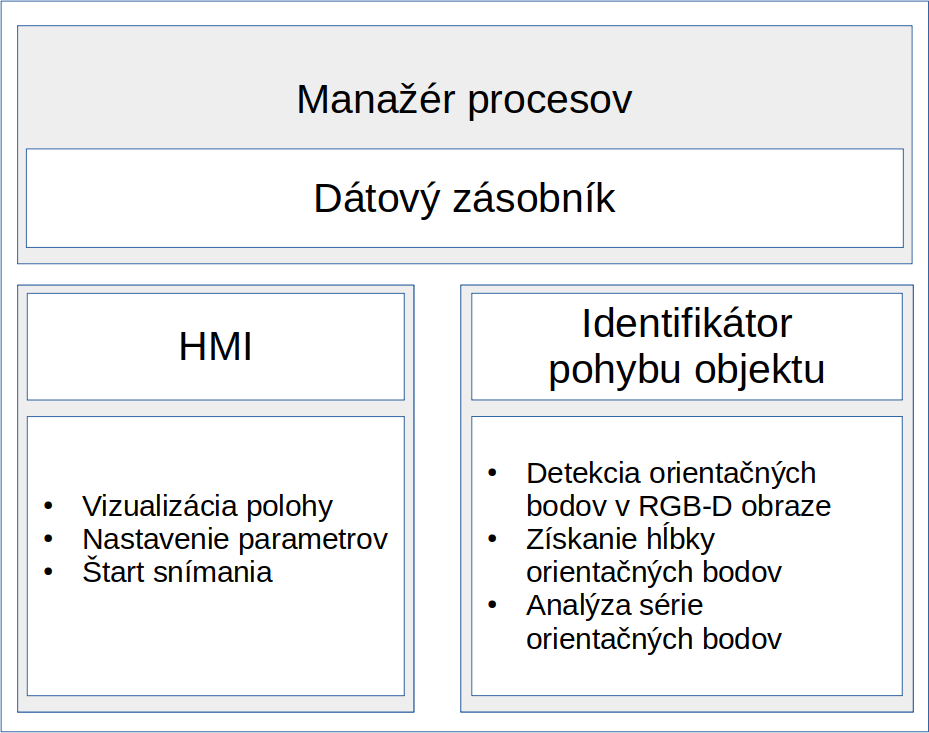
\includegraphics[width=0.75\textwidth]{figures/algorithm_faceland.png}
	\caption{Porovnanie vplyvu filtrácie na vstupné dáta}
	\label{fig:algorithm:result:a}
	\label{fig:algorithm:result:b}
	\label{fig:algorithm:result:c}
\end{figure}

\subsection{ICP registrácia}

\subsection{Segmentácia hĺbkovej mapy}
